\documentclass[11pt,]{article}
\usepackage{lmodern}
\usepackage{amssymb,amsmath}
\usepackage{ifxetex,ifluatex}
\usepackage{fixltx2e} % provides \textsubscript
\ifnum 0\ifxetex 1\fi\ifluatex 1\fi=0 % if pdftex
  \usepackage[T1]{fontenc}
  \usepackage[utf8]{inputenc}
\else % if luatex or xelatex
  \ifxetex
    \usepackage{mathspec}
  \else
    \usepackage{fontspec}
  \fi
  \defaultfontfeatures{Ligatures=TeX,Scale=MatchLowercase}
\fi
% use upquote if available, for straight quotes in verbatim environments
\IfFileExists{upquote.sty}{\usepackage{upquote}}{}
% use microtype if available
\IfFileExists{microtype.sty}{%
\usepackage{microtype}
\UseMicrotypeSet[protrusion]{basicmath} % disable protrusion for tt fonts
}{}
\usepackage[margin=1in]{geometry}
\usepackage{hyperref}
\hypersetup{unicode=true,
            pdftitle={Cartogram Mapping and its Application to Cancer Data Visualisation},
            pdfauthor={Stephanie Kobakian, Jessie Roberts and Dianne Cook},
            pdfborder={0 0 0},
            breaklinks=true}
\urlstyle{same}  % don't use monospace font for urls
\usepackage{longtable,booktabs}
\usepackage{graphicx,grffile}
\makeatletter
\def\maxwidth{\ifdim\Gin@nat@width>\linewidth\linewidth\else\Gin@nat@width\fi}
\def\maxheight{\ifdim\Gin@nat@height>\textheight\textheight\else\Gin@nat@height\fi}
\makeatother
% Scale images if necessary, so that they will not overflow the page
% margins by default, and it is still possible to overwrite the defaults
% using explicit options in \includegraphics[width, height, ...]{}
\setkeys{Gin}{width=\maxwidth,height=\maxheight,keepaspectratio}
\IfFileExists{parskip.sty}{%
\usepackage{parskip}
}{% else
\setlength{\parindent}{0pt}
\setlength{\parskip}{6pt plus 2pt minus 1pt}
}
\setlength{\emergencystretch}{3em}  % prevent overfull lines
\providecommand{\tightlist}{%
  \setlength{\itemsep}{0pt}\setlength{\parskip}{0pt}}
\setcounter{secnumdepth}{5}
% Redefines (sub)paragraphs to behave more like sections
\ifx\paragraph\undefined\else
\let\oldparagraph\paragraph
\renewcommand{\paragraph}[1]{\oldparagraph{#1}\mbox{}}
\fi
\ifx\subparagraph\undefined\else
\let\oldsubparagraph\subparagraph
\renewcommand{\subparagraph}[1]{\oldsubparagraph{#1}\mbox{}}
\fi

%%% Use protect on footnotes to avoid problems with footnotes in titles
\let\rmarkdownfootnote\footnote%
\def\footnote{\protect\rmarkdownfootnote}

%%% Change title format to be more compact
\usepackage{titling}

% Create subtitle command for use in maketitle
\providecommand{\subtitle}[1]{
  \posttitle{
    \begin{center}\large#1\end{center}
    }
}

\setlength{\droptitle}{-2em}

  \title{Cartogram Mapping and its Application to Cancer Data Visualisation}
    \pretitle{\vspace{\droptitle}\centering\huge}
  \posttitle{\par}
    \author{Stephanie Kobakian, Jessie Roberts and Dianne Cook}
    \preauthor{\centering\large\emph}
  \postauthor{\par}
    \date{}
    \predate{}\postdate{}
  

\begin{document}
\maketitle

{
\setcounter{tocdepth}{2}
\tableofcontents
}
\section*{Abstract}

Utilising maps to present statistics has been widely used for centuries.
These maps connect data and/or statistics to the geographical
representation of areas that are generally familiar to the audience.
However, it is not enough to be recognisable, if the meaning of the
statistic cannot be seen. This is particularly relevant to cancer
statistics, as cancer outcomes directly relate to the people living
within a geographical area. In situations where the people are of
interest, not the land they live on, it is reasonable to explore views
that enhance the communication of the cancer statistics. This has
spurred innovations over the previous centuries to enhance the shapes
and maps presented to effectively communicate cancer outcomes, and
health outcomes more broadly.

\hypertarget{introduction}{%
\section{Introduction}\label{introduction}}

\hypertarget{disease-mapping-methods}{%
\section{Disease mapping methods}\label{disease-mapping-methods}}

\hypertarget{current-best-practice-map-displays-for-cancer-data}{%
\subsection{Current best practice map displays for cancer
data}\label{current-best-practice-map-displays-for-cancer-data}}

A choropleth map is used to show the spatial relationship, or
variability, of measurements. Created as a storage device which
preserves locations for geographically ordered data, with usage dating
back to the 1800s (Berry, Morrill, and Tobler,
\protect\hyperlink{ref-GOINO}{n.d.}). They are constructed by drawing
the given geographic or political boundaries, and filling the shapes
with colours to represent values of a measured variable (Tufte
\protect\hyperlink{ref-EI}{1990}). Early versions used symbols or
patterns instead of colour. Bell et al.
(\protect\hyperlink{ref-CPISACA}{2006}) discusses the use of choropleth
maps for visualising cancer data, and Walter
(\protect\hyperlink{ref-DMAHP}{2001}) gives an overview of the
development of the use of choropleth maps for displaying disease data. A
choropleth map is a true map of the topology, constructed for visual
inspection of spatial patterns across a familiar geographic form. Figure
1 shows a choropleth map where each state of the United States of
America is coloured by the average annual rate of new cases of lung and
bronchus cancer from years 2012 to 2016.

\begin{figure}
\centering
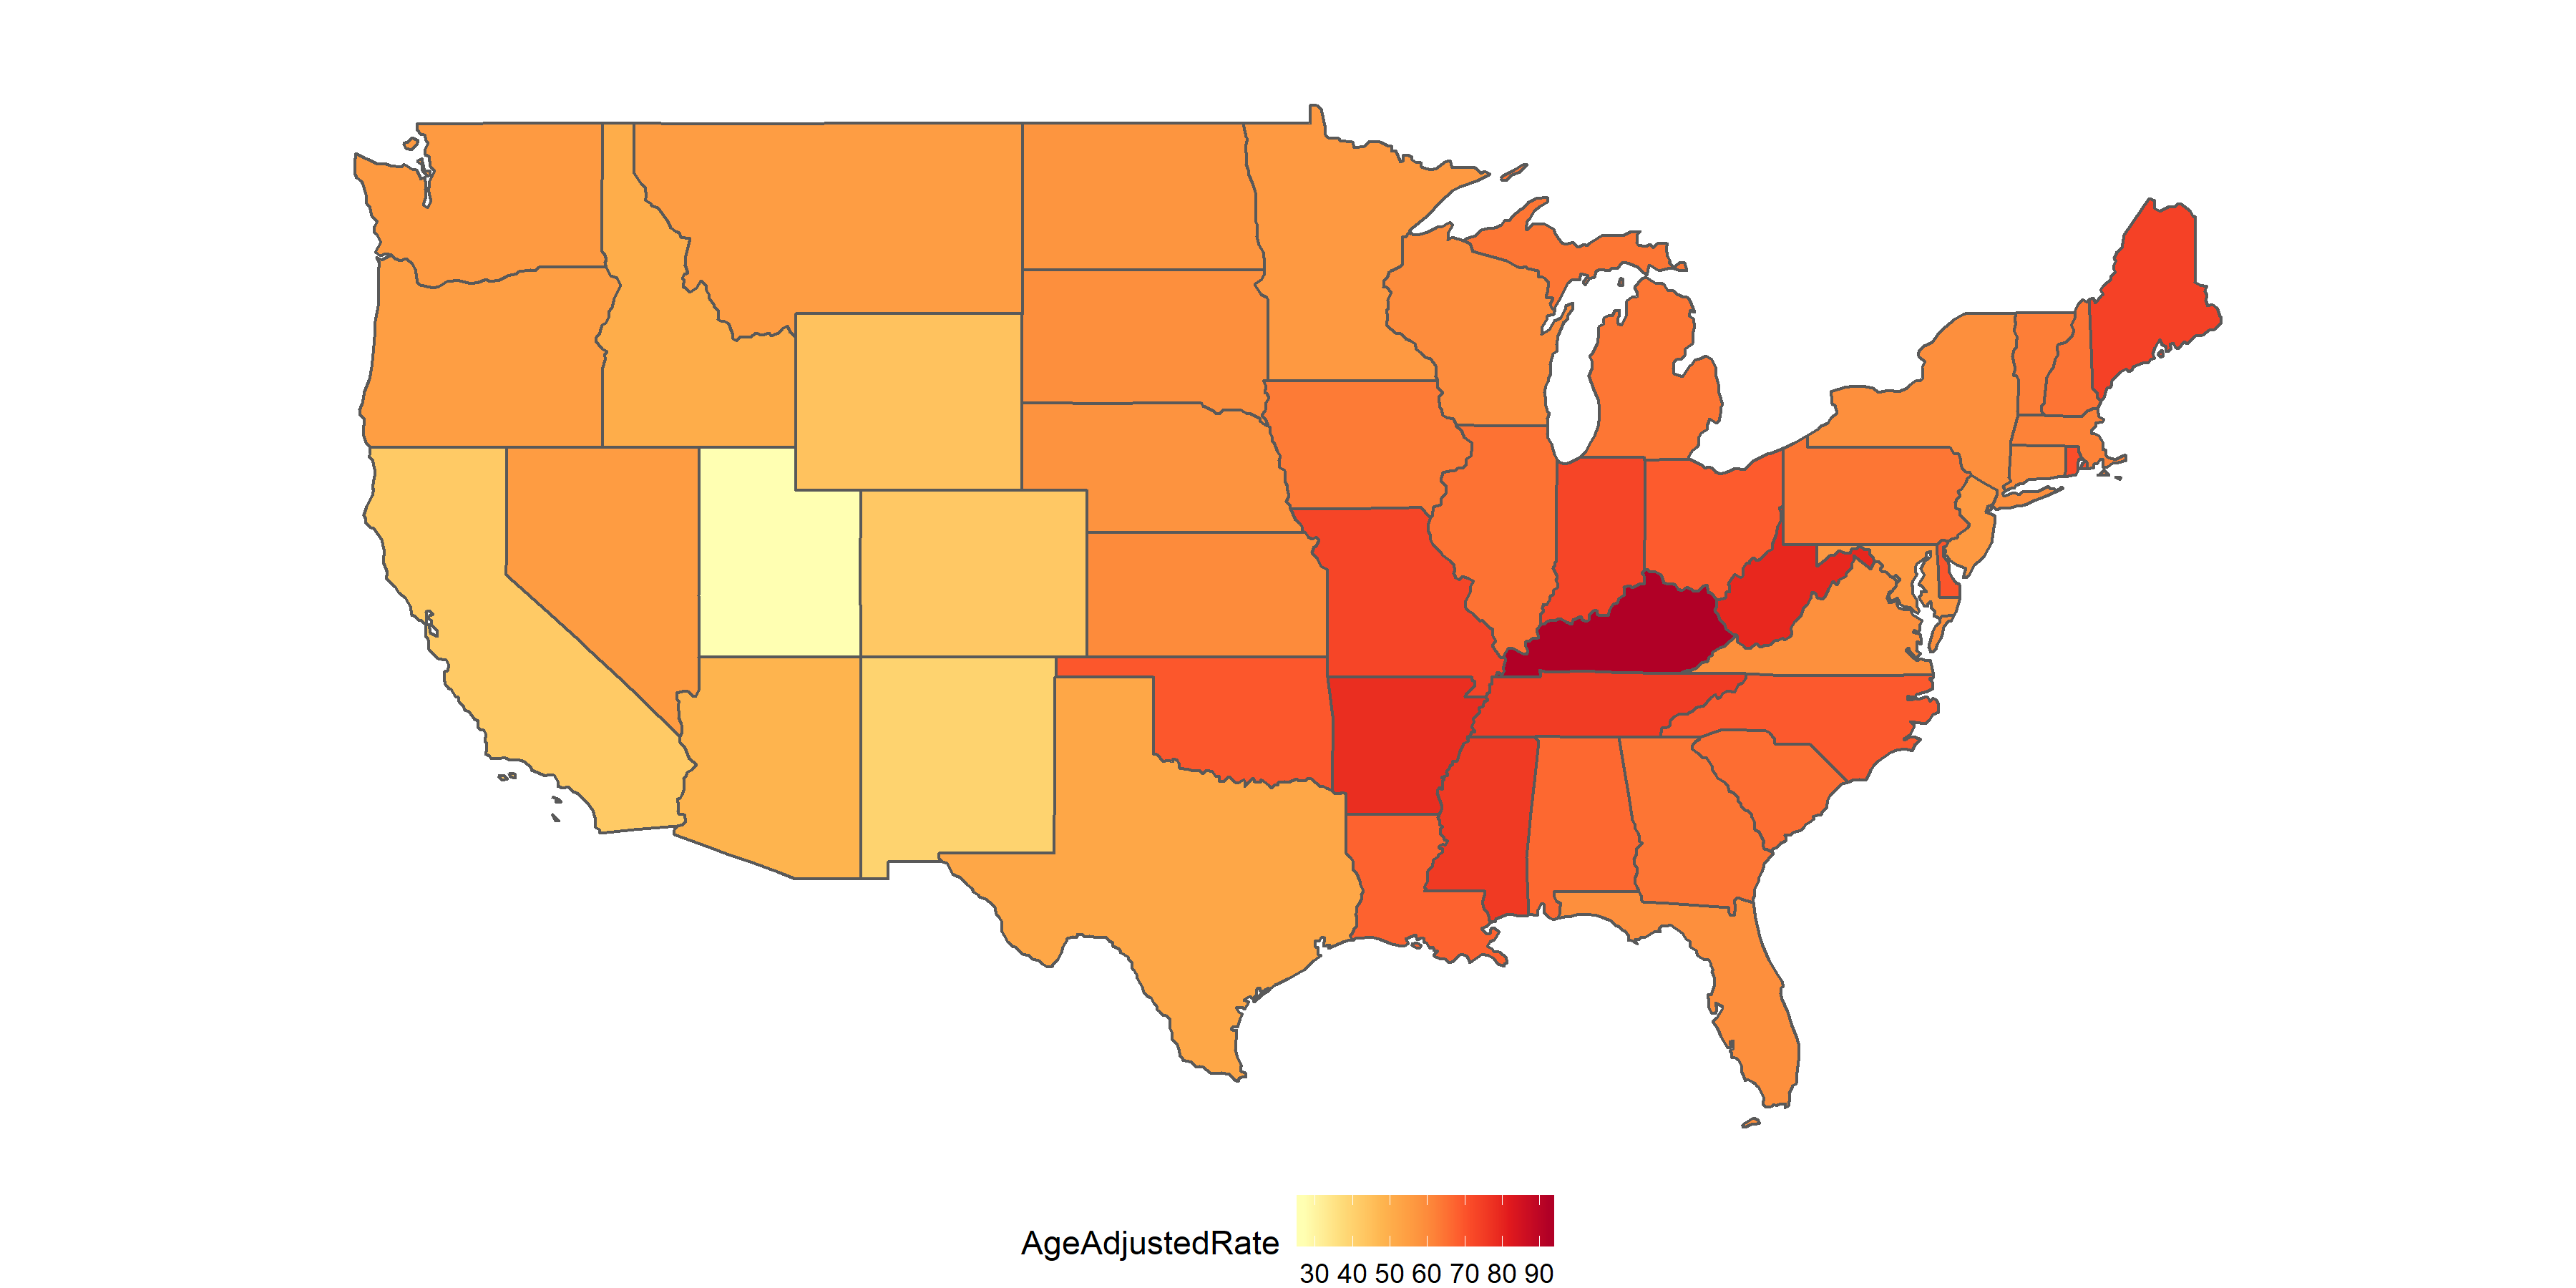
\includegraphics{figures/ggchoro.png}
\caption{``A choropleth map of the United States of America.''}
\end{figure}

Utilising the familiar state boundaries can make a map intuitive to read
(Brewster and Subramanian \protect\hyperlink{ref-CIBMUK}{2010}), and
allow viewers to visually infer the spatial relationships in the data,
i.e.~how cancer rate differs across the states. The familiarity of the
geography is a worthy consideration when presenting results of spatial
analysis. Just as geographers are no longer the only creators of maps,
Bell et al. (\protect\hyperlink{ref-CPISACA}{2006}) suggests the
audiences of spatial health data analysis have extended beyond
researchers to the public, policymakers and the media. However, while
the areas are recognisable shapes, they are often politically driven
boundaries with individual areas being of non-uniform size, containing
different population densities and subject to change over time. The
different population and geographical sizes of administrative areas can
attract attention to the shades of the unpopulated but large areas
(Tufte \protect\hyperlink{ref-EI}{1990}). Choropleths can inhibit visual
inference when presenting human related statistics as the display may
draw attention from the `potentially more important results in the more
populous communities' (Exeter \protect\hyperlink{ref-SE}{2017}).

In epidemiology, choropleths are often used as a tool to study the
spatial distribution of cancer incidence and mortality.

Almost 100 years of cancer mapping in the United States and the United
Kingdom has increased the effectiveness in the presentation of unbiased
rates. The increasing development and use of disease maps can be
attributed to the availability of geographic information system software
(Exeter \protect\hyperlink{ref-SE}{2017}). The data collection methods
of cancer mortality rates across regions, and administrative control
within regions lends itself to choropleth visualisation. Mortality rates
are now often presented as relative rates of risk across the population,
and age adjusted to correct for the the higher prevalence of cancers in
older populations. Howe (\protect\hyperlink{ref-HEDP}{1989}) describes
Stocks development of the standardised mortality ratios through the
1930s. The choropleth maps used at this time presented levels of cancer
via hatchings on a black and white scale.

Mortality rates are now often presented as relative rates of risk across
the population, and age adjusted. Howe
(\protect\hyperlink{ref-HEDP}{1989}) describes Stocks' development of
the standardised mortality ratios through the 1930s. The choropleth maps
used presented levels of cancer via hatchings on a black and white
scale.

Examples of atlases: Kraak 1998, Kraak and Ormeling 2011 Bertin 1967

\hypertarget{public-face}{%
\subsection{Public face}\label{public-face}}

A grey literature review conducted by (ref) identified 33 publicly
available cancer atlases published on the internet between 01/01/2010 to
11/11/2015. Reflecting the high use of chloropleth maps founds in the
literature, outlined in the section above, all the public facing maps
identified in this review were also chloropleth maps.

\hypertarget{publishers}{%
\subsubsection*{Publishers}\label{publishers}}
\addcontentsline{toc}{subsubsection}{Publishers}

The majority of atlases were published by non-commercial organisations,
including not-for-profits (NFPs), government, research organisations,
advocacy groups or a partnership between an NFP \& government. Only one
map was published by a commercial entity (Maps of Cancer Mortality Rates
in Spain), in this case a media organisation El Pais\footnote{\url{https://elpais.com/}}.

\hypertarget{reported-measures}{%
\subsubsection*{Reported measures}\label{reported-measures}}
\addcontentsline{toc}{subsubsection}{Reported measures}

The majority of maps identified in this study reported age adjusted
rates of either incidence, mortality or survival. The list below
summarises these measures, and provides a definition of each measure.

\hypertarget{geographical-coverage}{%
\subsubsection*{Geographical coverage}\label{geographical-coverage}}
\addcontentsline{toc}{subsubsection}{Geographical coverage}

Identified cancer atlases covered geographies from all around the world:
4 were global, 3 from Australia (AUS), 11 from the United States (US), 2
from Canada (CAN), 7 from the United Kingdom (UK), 2 from Spain, 1 from
Switzerland, 1 from Germany, 1 from Norway, and 1 covering the European
Union. Not all maps had a national focus and 10 covered a region or
state rather than an entire nation. The states or counties/regions
covered were South Australia (AUS), Queensland (AUS), Ontario (CAN),
Valencia (Spain), Pennsylvania county Massachusetts (US), New Hampshire
(US), Cape Cod (US), Missouri (US), Florida (US), New York State (US)
and Arizona (US).

\newpage

\begin{longtable}[]{@{}ll@{}}
\caption{(\#tab:measures) Measures used to report cancer
statistics}\tabularnewline
\toprule
\begin{minipage}[b]{0.28\columnwidth}\raggedright
Measure\strut
\end{minipage} & \begin{minipage}[b]{0.66\columnwidth}\raggedright
Details\strut
\end{minipage}\tabularnewline
\midrule
\endfirsthead
\toprule
\begin{minipage}[b]{0.28\columnwidth}\raggedright
Measure\strut
\end{minipage} & \begin{minipage}[b]{0.66\columnwidth}\raggedright
Details\strut
\end{minipage}\tabularnewline
\midrule
\endhead
\begin{minipage}[t]{0.28\columnwidth}\raggedright
1. IR (Incidence Ratio)\strut
\end{minipage} & \begin{minipage}[t]{0.66\columnwidth}\raggedright
\((IR)_i=\frac{(Incidence\ Rate)_i}{Average\ Incidence\ Rate}\),\strut
\end{minipage}\tabularnewline
\begin{minipage}[t]{0.28\columnwidth}\raggedright
\strut
\end{minipage} & \begin{minipage}[t]{0.66\columnwidth}\raggedright
Cancer incidence rate in region \(i\) over the average cancer incidence
rate for the total region\strut
\end{minipage}\tabularnewline
\begin{minipage}[t]{0.28\columnwidth}\raggedright
2. SIR (Standardised Incidence Ratio)\strut
\end{minipage} & \begin{minipage}[t]{0.66\columnwidth}\raggedright
IR standardised by age structure in each region \(i\)\strut
\end{minipage}\tabularnewline
\begin{minipage}[t]{0.28\columnwidth}\raggedright
3. RER\strut
\end{minipage} & \begin{minipage}[t]{0.66\columnwidth}\raggedright
\(RER = \frac{(Cancer\ related\ mortality)_i}{Average\ cancer\ related\ mortality}\)\strut
\end{minipage}\tabularnewline
\begin{minipage}[t]{0.28\columnwidth}\raggedright
(Relative Excess Risk)\strut
\end{minipage} & \begin{minipage}[t]{0.66\columnwidth}\raggedright
Represents the estimate of cancer related mortality within five years of
diagnosis\strut
\end{minipage}\tabularnewline
\begin{minipage}[t]{0.28\columnwidth}\raggedright
\strut
\end{minipage} & \begin{minipage}[t]{0.66\columnwidth}\raggedright
Also referred to as `excess hazard ratio'\strut
\end{minipage}\tabularnewline
\begin{minipage}[t]{0.28\columnwidth}\raggedright
4. Age Adjusted Relative Risk\strut
\end{minipage} & \begin{minipage}[t]{0.66\columnwidth}\raggedright
RR standardised by age structure in each region \(i\)\strut
\end{minipage}\tabularnewline
\begin{minipage}[t]{0.28\columnwidth}\raggedright
5. Rate per 100,000\strut
\end{minipage} & \begin{minipage}[t]{0.66\columnwidth}\raggedright
Cancer incidence per 100,000 population\strut
\end{minipage}\tabularnewline
\begin{minipage}[t]{0.28\columnwidth}\raggedright
6. Age Adjusted Rate per 100,000\strut
\end{minipage} & \begin{minipage}[t]{0.66\columnwidth}\raggedright
\#5 standardised by age structure or region\strut
\end{minipage}\tabularnewline
\begin{minipage}[t]{0.28\columnwidth}\raggedright
7. New cancer cases per 100,000\strut
\end{minipage} & \begin{minipage}[t]{0.66\columnwidth}\raggedright
Specific methods could not be found\strut
\end{minipage}\tabularnewline
\begin{minipage}[t]{0.28\columnwidth}\raggedright
8. Count\strut
\end{minipage} & \begin{minipage}[t]{0.66\columnwidth}\raggedright
Crude cancer counts\strut
\end{minipage}\tabularnewline
\begin{minipage}[t]{0.28\columnwidth}\raggedright
9. Below or above Expected\strut
\end{minipage} & \begin{minipage}[t]{0.66\columnwidth}\raggedright
Alternative expression of the SIR\strut
\end{minipage}\tabularnewline
\bottomrule
\end{longtable}

\hypertarget{statistical-uncertainty}{%
\subsubsection{Statistical uncertainty}\label{statistical-uncertainty}}

Cancer atlases were considered to report uncertainty to the non-expert
user if they included a measure of statistical uncertainty either within
or alongside the map. Maps that only reported this information within
the supplementary material were not considered to have directly
attempted to report uncertainty.

The review did not reveal any novel uncertainty visualisation approaches
or visualisations. Maps used standard and well known measures including
credible intervals and standard deviation, statistical significance, box
plots and distributions. These maps ranged from static pdfs or
infographics to interactive online resources. The interactivity of the
more modern maps enabled uncertainty information to be incorporated
without cluttering the screen, such as in a tool tip feature.

\begin{figure}

{\centering 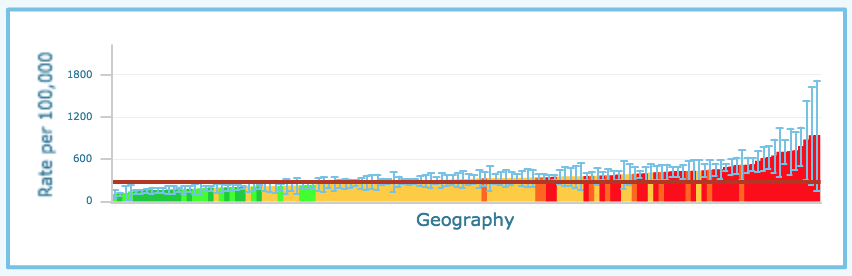
\includegraphics[width=0.8\linewidth]{figures/Alberta_CI_viz} 

}

\caption{Example of CI visualisation for uncertainty representation in cancer mapping (1/3). Source: Alberta Health IHDA Geographic. (2012) }\label{fig:ci-viz2}
\end{figure}

\begin{figure}

{\centering 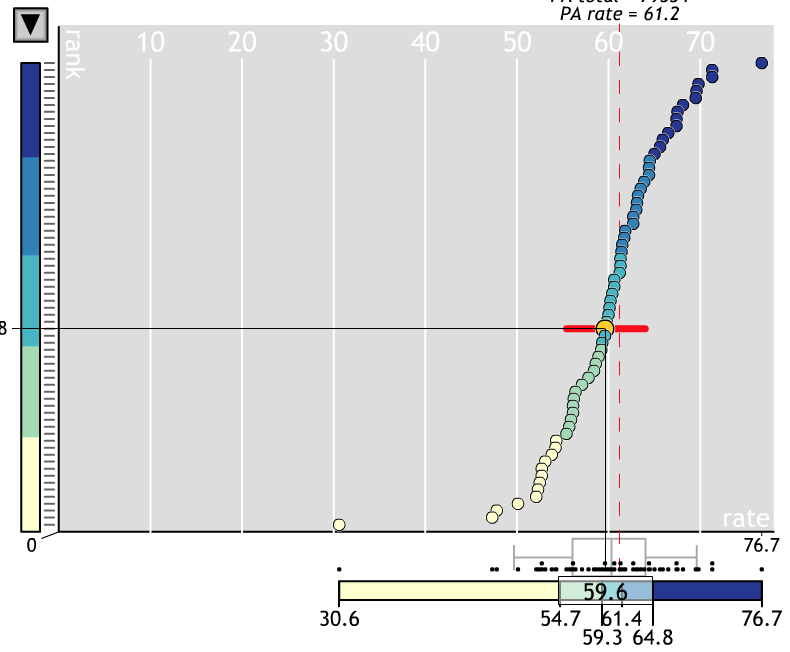
\includegraphics[width=0.55\linewidth]{figures/Pennsylvania_CI_viz} 

}

\caption{Example of CI visualisation for uncertainty representation in cancer mapping (2/3). Source: Pensylvania Cancer Atlas }\label{fig:ci-viz3}
\end{figure}

Close to half of the atlases identified (42\%, n=14) included some
measure of uncertainty. The most common measure used to represent
uncertainty were credible or confidence intervals (CIs). CIs were either
visualised by including their bounds in a scatterplot or graph of
estimates vs region (see Figures @ref(fig:ci-viz2)\footnote{Alberta
  Health IHDA Geographic. (2012). Age-Standardised Incidence Rate of
  COPD, 2011. Retrieved from:
  \url{http://www.health.alberta.ca/health-info/IHDA-geographic/COPD/incidence-agestandard/atlas.html?epik=0GJSpE_IW34lx}},
and @ref(fig:ci-viz3)\footnote{Centres for Disease Control and
  Prevention (CDC). (n.d). United States Cancer Statistics: An
  Interactive Cancer Atlas (InCA). Retrieved
  from:\url{https://nccd.cdc.gov/DCPC_INCA/}} positioned next to the
map, or reported numerically through the CI upper and lower bounds
listed in a data table (see Figure 3.4\footnote{Pennsylvania Cancer
  Atlas. (n.d). Retrieved from:
  \url{https://www.geovista.psu.edu/grants/CDC/?epik=0lJSpE_IW34lx}}).
Of those that visualised the CIs, 30\% (n=10) embedded the visualisation
within a tool tip function which visualised the CI when the mouse
hovered over the relevant area (see Figure 3.5\footnote{International
  Agency for Research on Cancer. (2017). Atlas of Cancer Mortality in
  the European Union and European Economic Area 1993-1997, Annex 4 -
  Cancer mortality maps by site. Retrieved from:
  \url{http://www.iarc.fr/en/publications/pdfs-online/epi/sp159/}}).

\begin{figure}

{\centering 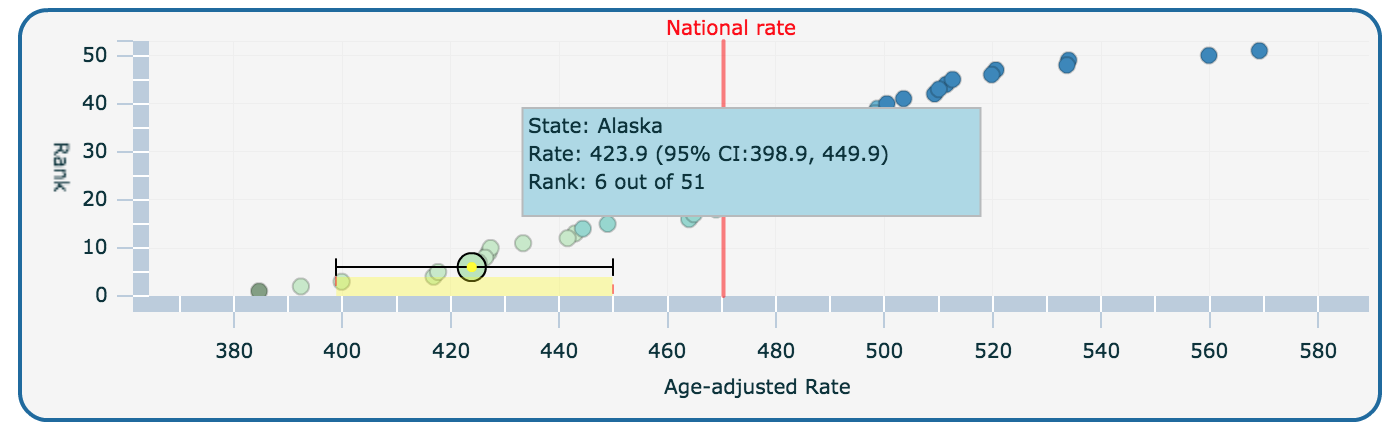
\includegraphics[width=0.6\linewidth]{figures/CDC_CI_viz_tooltip} 

}

\caption{Example of CI visualisation for uncertainty representation in cancer mapping (3/3). Source: Centres for Disease Control and Prevention (CDC). United States Cancer Statistics: An Interactive Cancer Atlas (InCA) }\label{fig:ci-tooltip}
\end{figure}

\begin{figure}

{\centering 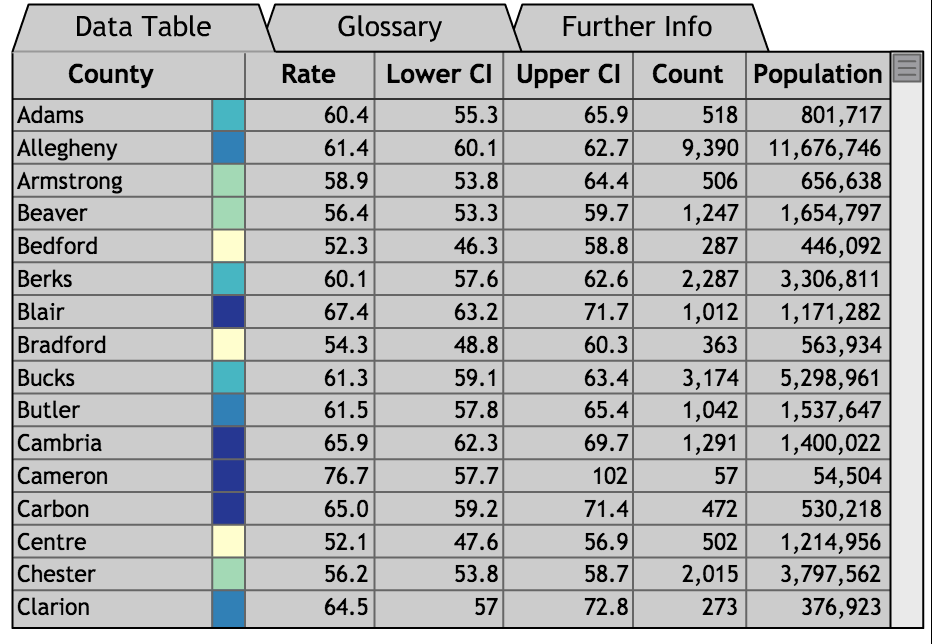
\includegraphics[width=0.5\linewidth]{figures/uncert_table} 

}

\caption{Example of an interactive data table with CI upper and lower bounds used in cancer mapping. Source: Pennsylvania Cancer Atlas}\label{fig:ci-table}
\end{figure}

Methods for representing sources of uncertainty information can be
visualised or communicated in different ways, examples identified
through this grey literature review are listed below.

\begin{figure}

{\centering 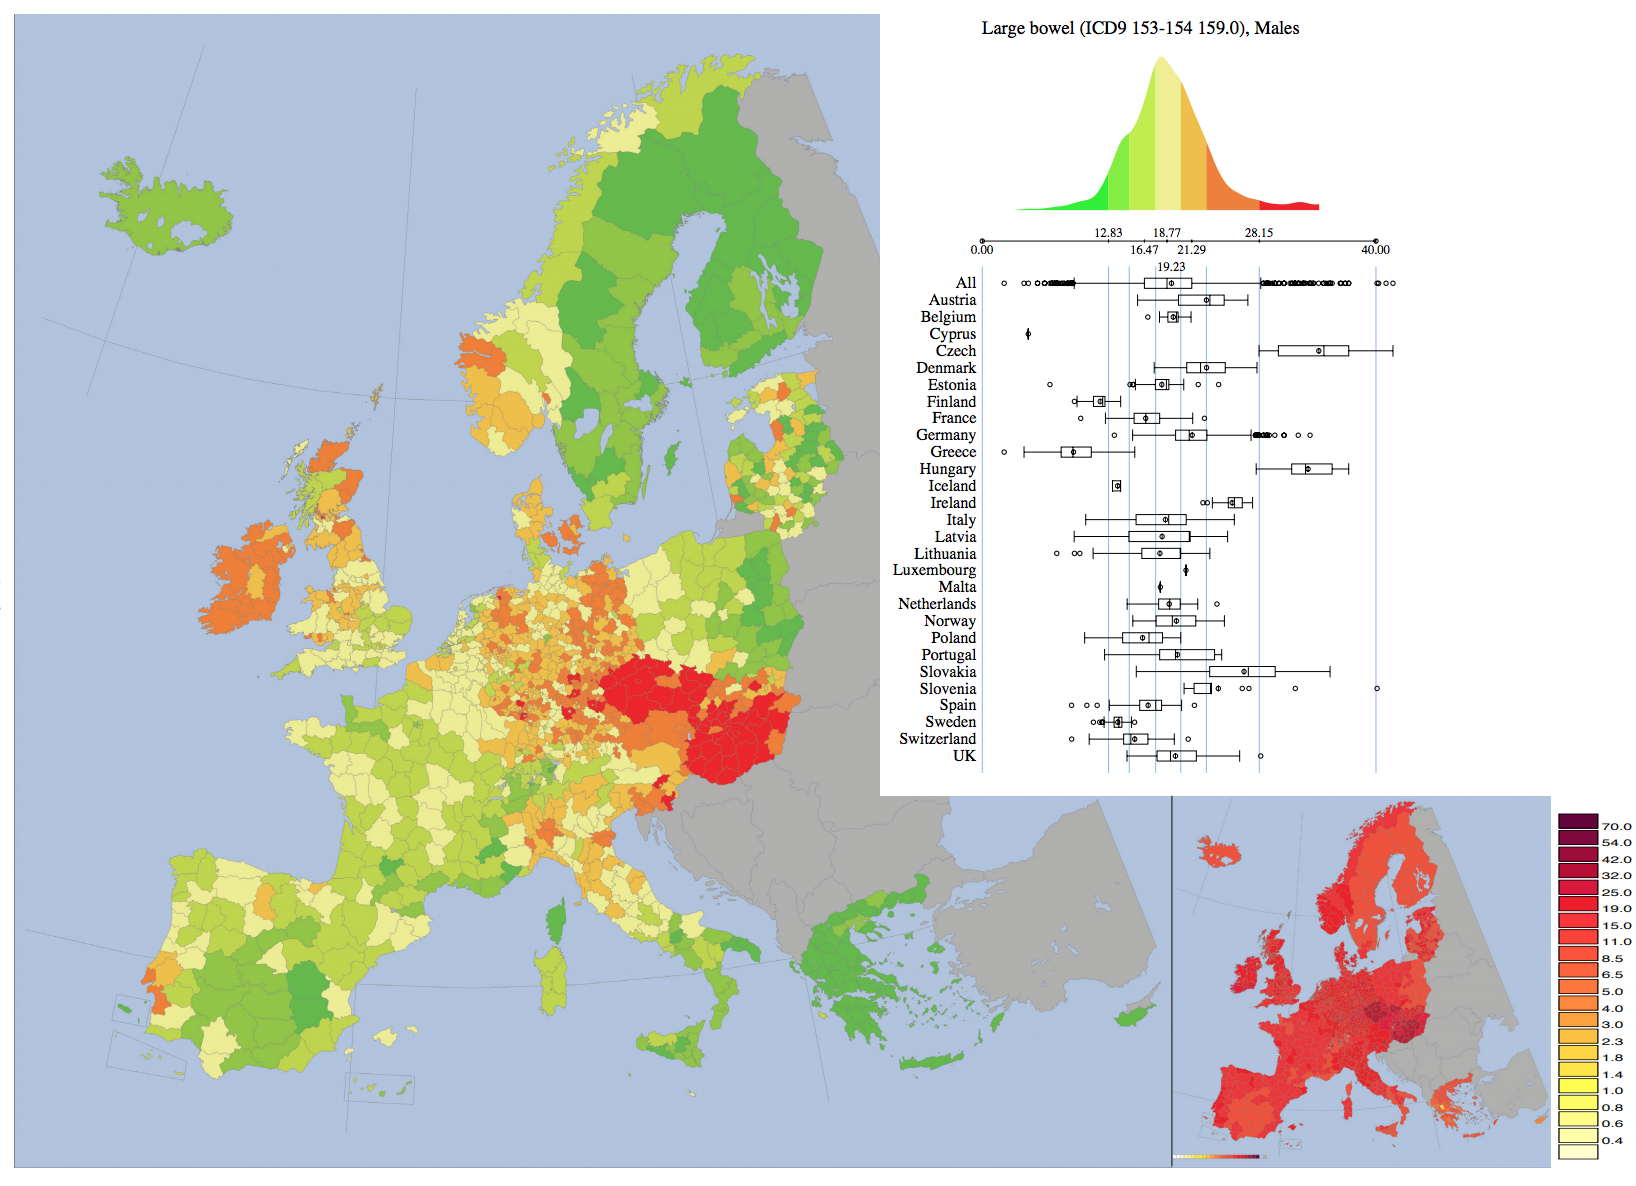
\includegraphics[width=0.9\linewidth]{figures/standard_deviation_large} 

}

\caption{Example of standard deviation visualised in cancer mapping}\label{fig:stndvn-example}
\end{figure}

\begin{figure}

{\centering 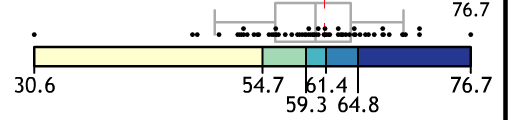
\includegraphics[width=0.4\linewidth]{figures/Boxplot2} 

}

\caption{Example of boxplot used in cancer mapping. Source: Source: Pensylvania Cancer Atlas }\label{fig:boxplot-example}
\end{figure}

\begin{longtable}[]{@{}ll@{}}
\caption{(\#tab:method-exp) Implicit and explicit measures of
uncertainty.}\tabularnewline
\toprule
\begin{minipage}[b]{0.35\columnwidth}\raggedright
Measure\strut
\end{minipage} & \begin{minipage}[b]{0.59\columnwidth}\raggedright
Example\strut
\end{minipage}\tabularnewline
\midrule
\endfirsthead
\toprule
\begin{minipage}[b]{0.35\columnwidth}\raggedright
Measure\strut
\end{minipage} & \begin{minipage}[b]{0.59\columnwidth}\raggedright
Example\strut
\end{minipage}\tabularnewline
\midrule
\endhead
\begin{minipage}[t]{0.35\columnwidth}\raggedright
CI Interval\strut
\end{minipage} & \begin{minipage}[t]{0.59\columnwidth}\raggedright
Figures 3.1, 3.2, 3.3\strut
\end{minipage}\tabularnewline
\begin{minipage}[t]{0.35\columnwidth}\raggedright
Statistical Significance\strut
\end{minipage} & \begin{minipage}[t]{0.59\columnwidth}\raggedright
Textured overlay on top of coloured regions used to indicate statistical
significance\strut
\end{minipage}\tabularnewline
\begin{minipage}[t]{0.35\columnwidth}\raggedright
Distribution\strut
\end{minipage} & \begin{minipage}[t]{0.59\columnwidth}\raggedright
Figure 3.4\strut
\end{minipage}\tabularnewline
\begin{minipage}[t]{0.35\columnwidth}\raggedright
Boxplots\strut
\end{minipage} & \begin{minipage}[t]{0.59\columnwidth}\raggedright
Figures 3.4, 3.5\strut
\end{minipage}\tabularnewline
\begin{minipage}[t]{0.35\columnwidth}\raggedright
Sample Size\strut
\end{minipage} & \begin{minipage}[t]{0.59\columnwidth}\raggedright
Textured overlay or lack of colour on a region, was used to show regions
with small sample size\strut
\end{minipage}\tabularnewline
\begin{minipage}[t]{0.35\columnwidth}\raggedright
Standard deviation\strut
\end{minipage} & \begin{minipage}[t]{0.59\columnwidth}\raggedright
Figure 3.6 - the second map in the bottom right corner shows standard
deviation\strut
\end{minipage}\tabularnewline
\bottomrule
\end{longtable}

\hypertarget{cartograms}{%
\subsection{Cartograms}\label{cartograms}}

Choropleths may be considered true topological maps, however, if the
land mass presented covers enough of the globe, there must be a
transformation or distortion to display in 2D. The amount of distortion
is related to the distance displayed Tobler
(\protect\hyperlink{ref-GAMP}{1963}). The world projections reflect the
frequent distortions seen from altering perspectives. Choropleth maps
will always be distorted if they cover enough of the globe, as will
photographs of the globe from space. Choropleth creation requires
choosing a map projection that shows a favourable distortion of the
geography for presenting the set of spatial information. Diagrams that
do not specify a projection can be considered to have some unknown
projection.

\begin{figure}
\centering
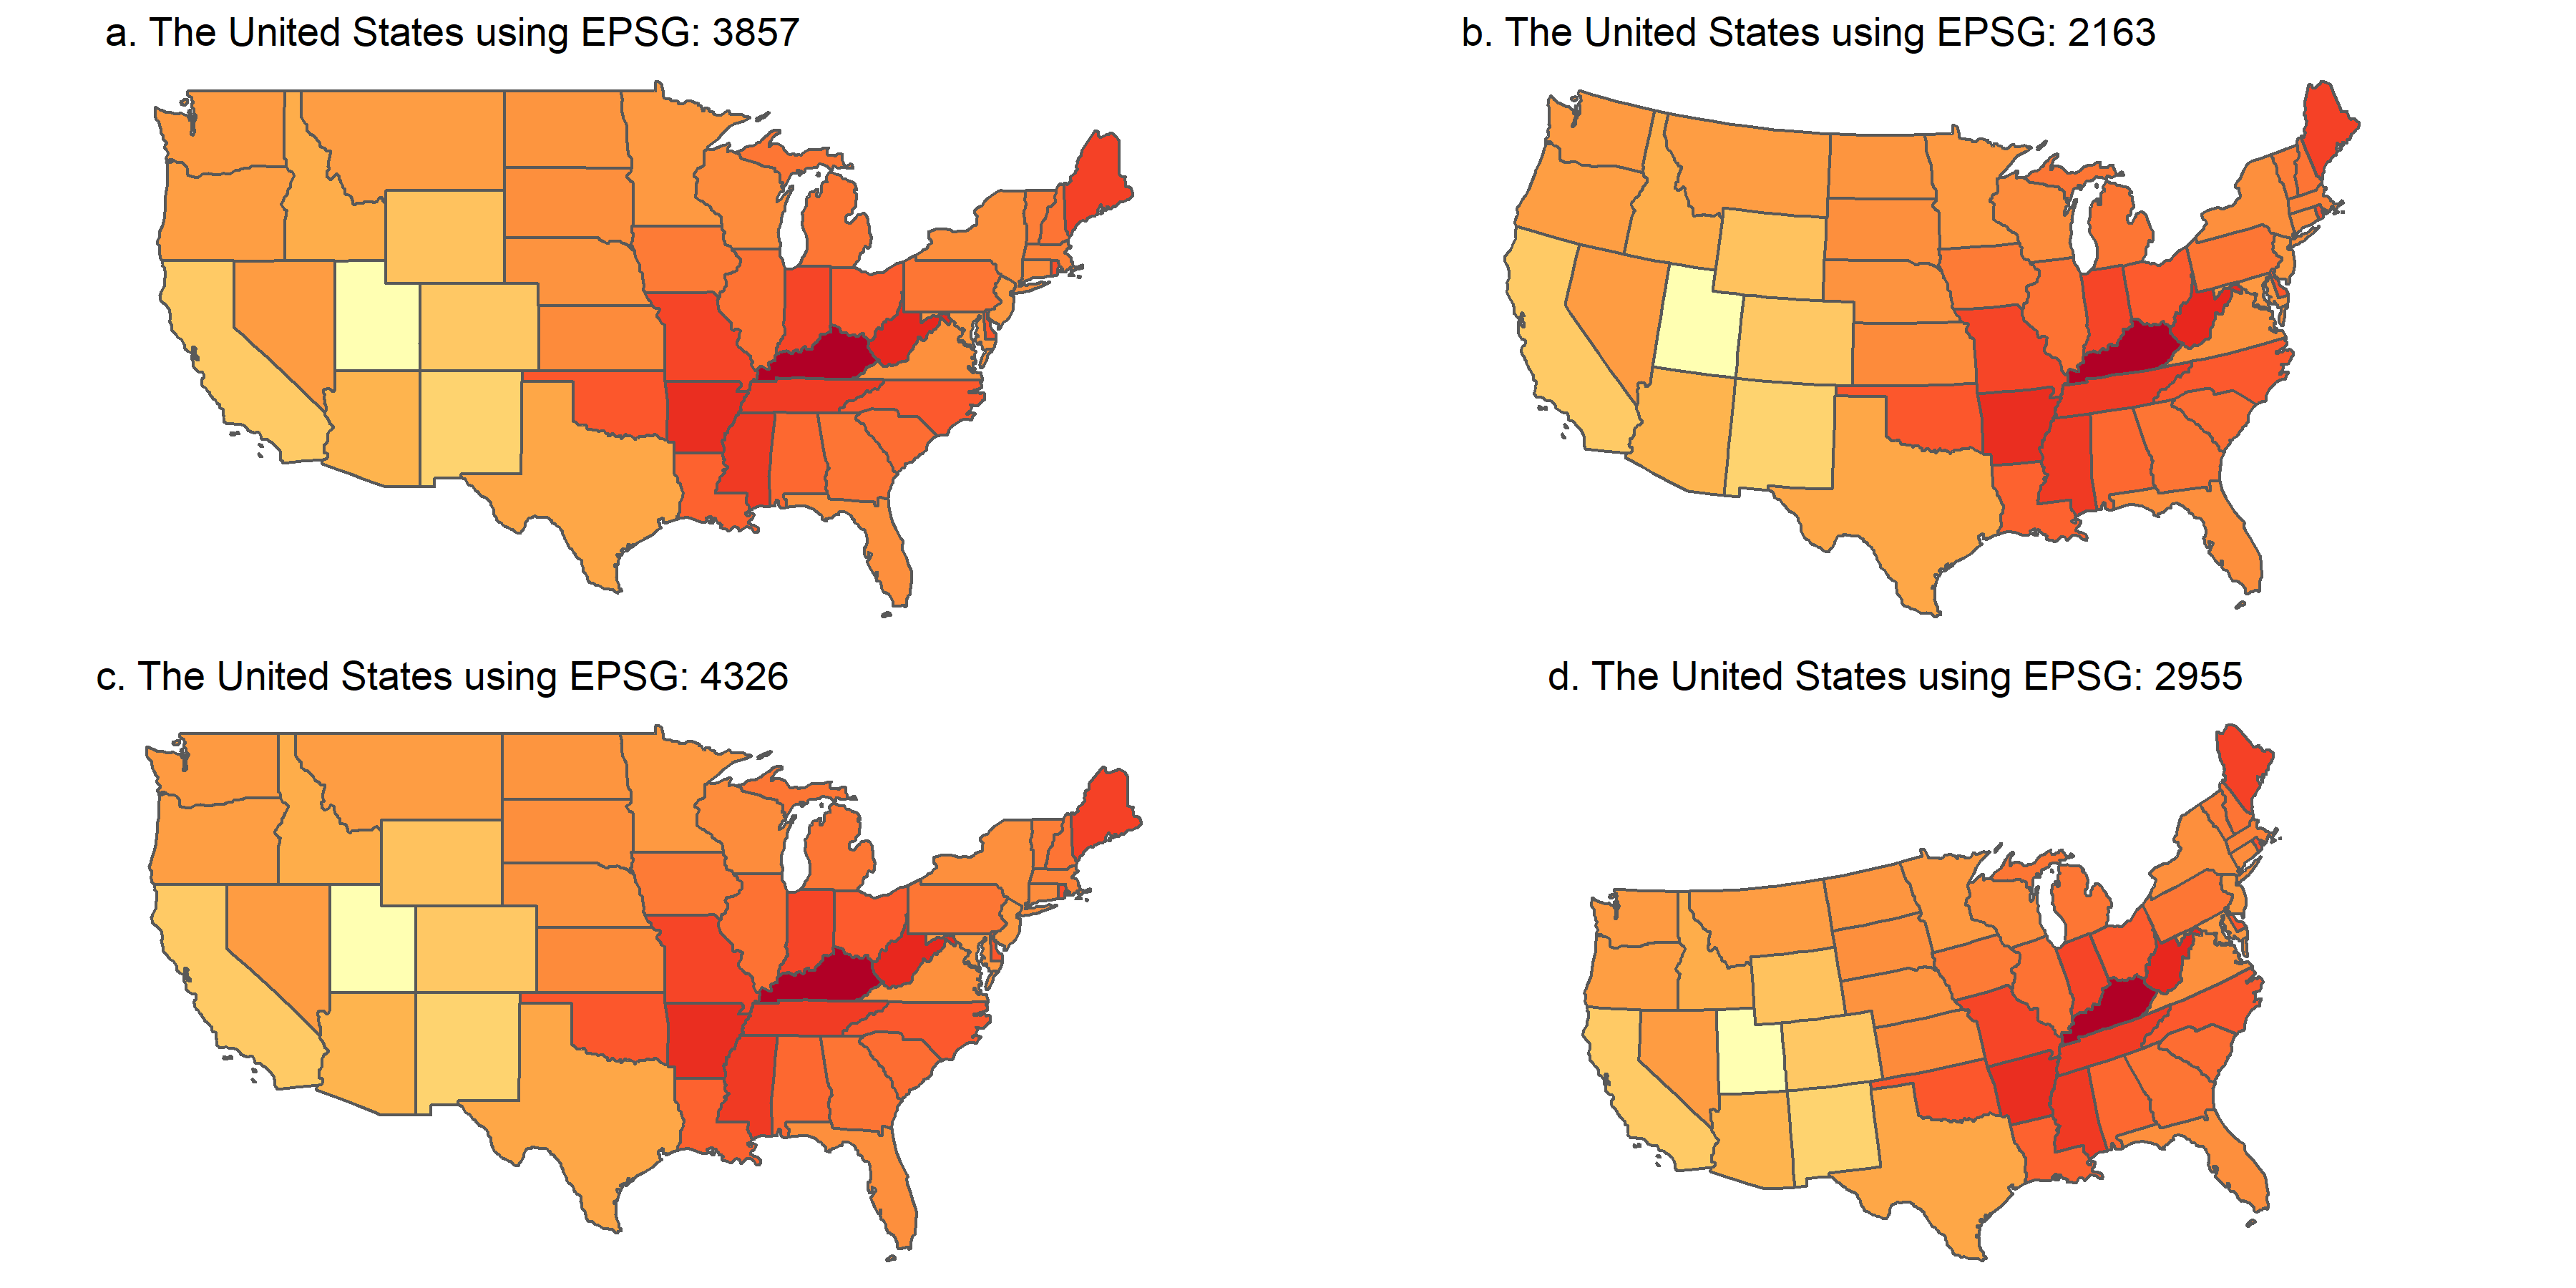
\includegraphics{figures/ggchoroCRS.png}
\caption{``Choropleth maps of the United States of America using four
coordinate reference systems.''}
\end{figure}

Waldo Tobler (\protect\hyperlink{ref-TVSSS}{2012}) explores many
graphical techniques, and suggests there are particular methods for
particular purposes. Cartograms provide an alternative visualisation
method for statistical and geographical information. The key difference
between a choropleth and a cartogram is the desirable augmentation of
the size, shape or distance of geographical areas (Dorling
\protect\hyperlink{ref-ACTUC}{2011}). Cartograms may be seen as an
extension of map transformations and projections. The favourable
distortion is proportional to a value other other than actual earth size
area (Olson \protect\hyperlink{ref-NAC}{1976}).

Using choropleth maps for population characteristics requires graphic
distortions when the population concerned varies greatly in density
(Griffin \protect\hyperlink{ref-CTTMB}{1980}). When implementing a
distortion of the geographical shape according to population, an area
cartogram (Olson \protect\hyperlink{ref-NAC}{1976}), or iso-demographic
map is the result. When visualising population statistics Dorling
(\protect\hyperlink{ref-ACTUC}{2011}) considers this equitable
representation design `more socially just, giving due attention to all
members of the population and reducing the visual impact of large areas
with small populations (Walter \protect\hyperlink{ref-DMAHP}{2001}).
Griffin (\protect\hyperlink{ref-CTTMB}{1980}) suggest that spatial
socio-economic data is best presented on a cartogram for urban areas.
Howe (\protect\hyperlink{ref-HEDP}{1989}) agrees that 'cancer occurs in
people, not in geographical areas' and the map bases of population
reflect this and avoid allocating `undue prominence' to rural areas.
Jahan et al. (\protect\hyperlink{ref-MTMSIH}{2018}) encourage the use of
cartograms to highlight small areas and uncover local-level
inequalities. Using health estimates from large areas can prevent
drawing attention to the inequalities.

The area on the map space can also be used represent a value. There have
been many algorithms presented, Nusrat and Kobourov
(\protect\hyperlink{ref-SAIC}{2016}) provided a framework to investigate
implementations and the ``statistical accuracy, geographical accuracy,
and topological accuracy''. The spatial transformation of map regions
relative to the data emphasises the data distribution instead of land
size (Kocmoud and House \protect\hyperlink{ref-CBATCC}{1998}).

Cancer statistics and atlases

The creation of cartograms was largely in the hands of cartographers.
Dorling (\protect\hyperlink{ref-ACTUC}{2011}) discusses early approaches
including John Hunter and Jonathan Young (1968) and Durham's wooden tile
method, Skoda and Robertson's (1972) steel ball bearing approach and
Tobler's (1973) computer programs.

There are many alternatives to consider, the intended audience of the
map, and its purpose are key points in cartogram use and creation.
Dorling (\protect\hyperlink{ref-ACTUC}{2011}) reiterates: `There is no
``best'' cartogram or method of creating cartograms just as there is no
``best'' map' (Monmonier and Schnell, 1988).

`Firstly, that no such transformation has a unique solution, leaving the
subjective choice in the hands of the individual map designer.'

Design goals: - to maintain as much as possible of the intricate detail
- to maximize the simplicity of the transformation - maintenance of
directional accuracy - attempt to influence and direct the map user's
attention,

\begin{enumerate}
\def\labelenumi{\arabic{enumi})}
\tightlist
\item
  that the size of the electoral subdivisions should be made
  proportional to their respective electoral populations,
\item
  that the contiguity relationships between the DCU's should be
  maintained,
\item
  that true directions should be retained from the centre of the
  transformation,
\item
  that the main shape characteristics of the DCU's should be preserved,
  and
\item
  that the map should possess the overall shape of the built-up area.
\end{enumerate}

\hypertarget{contiguous}{%
\subsubsection{Contiguous}\label{contiguous}}

\begin{figure}
\centering
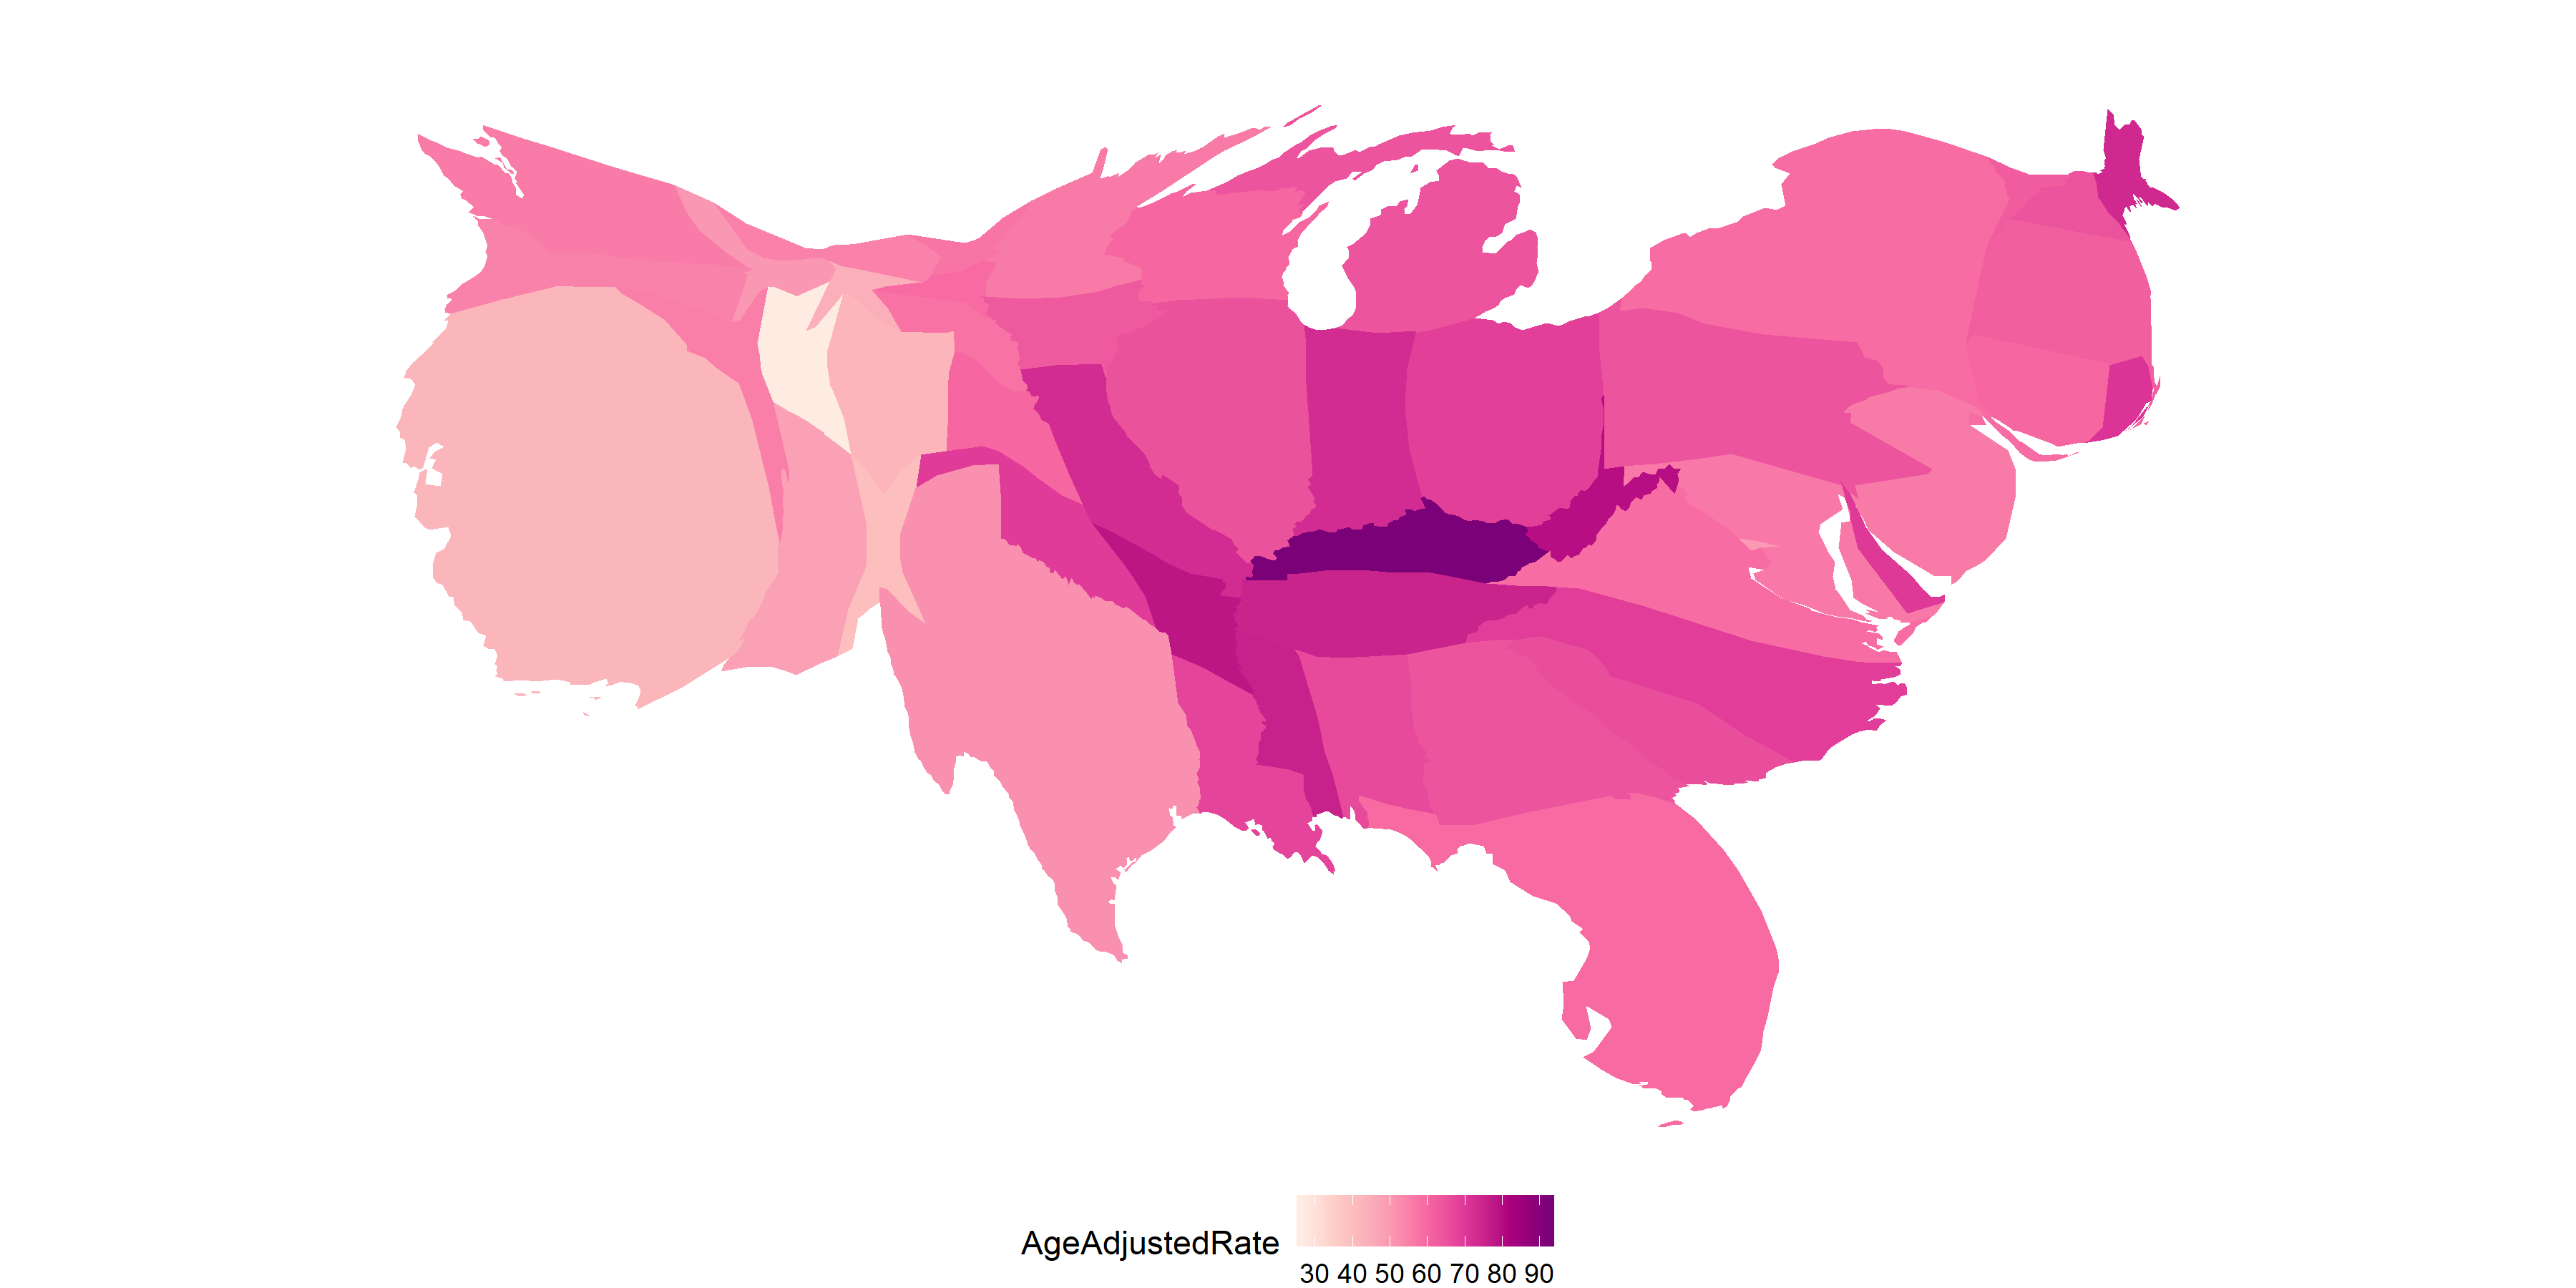
\includegraphics{figures/ggcont.png}
\caption{``A contiguous cartogram of the Unites States of America''}
\end{figure}

A contiguous cartogram allows the map space to highlight the
distribution of the variable. These cartograms maintain connectivity of
the map regions while areas are resized according to a statistic, this
often must occur at the expense of the shape (Kocmoud and House
\protect\hyperlink{ref-CBATCC}{1998},@NAC, @TAAM). From a computer
graphics perspective, Min Ouyang and Revesz
(\protect\hyperlink{ref-ACA}{2000}) believe it is a problem of `map
deformation' to account for the value assigned to each area, they
provide three methods for creating value-by-area cartograms. Examples
include Tobler's Pseudo-Cartogram Method, Dorling's Cellular Automaton
Method (\protect\hyperlink{ref-ACTUC}{2011}), Radial Expansion Method of
Selvin et al., Rubber Sheet Method of Dougenik et al., Gusein-Zade and
Tikunov's Line Integral Method, Constraint-Based Method (Kocmoud and
House) (\protect\hyperlink{ref-CBATCC}{1998}).

describes the process of creating a population cartogram for Canada,
using the 1966 Census. An intentional goal of this project was to
maintain contiguity, while attempting to keep the actual shape of
places. The end result was a `very accurate isodemo-graphic map of
Canada'. This intentional design goal coincided with the rising interest
in urban geography.

To be able to recognise the significant changes, a reader will usually
have to know the initial geography to find the differences in the new
cartogram layout (Olson \protect\hyperlink{ref-NAC}{1976}). Tobler's
Conformal mapping means to preserve angles locally so that the shapes of
very small areas on a traditional map and a cartogram would be similar.
Kocmoud and House (\protect\hyperlink{ref-CBATCC}{1998}) presents this
issue as conflicting tasks or aims, to adjust region sizes and retain
region shapes. Distortion of region shapes on the contiguous cartogram
presents an additional hurdle to visual recognition and this hurdle is
not only eliminated on the noncontiguous cartogram but is replaced by
the meaningful empty-space property (Olson
\protect\hyperlink{ref-NAC}{1976}, @ECGC).

\hypertarget{non-contiguous}{%
\subsubsection{Non-Contiguous}\label{non-contiguous}}

\begin{figure}
\centering
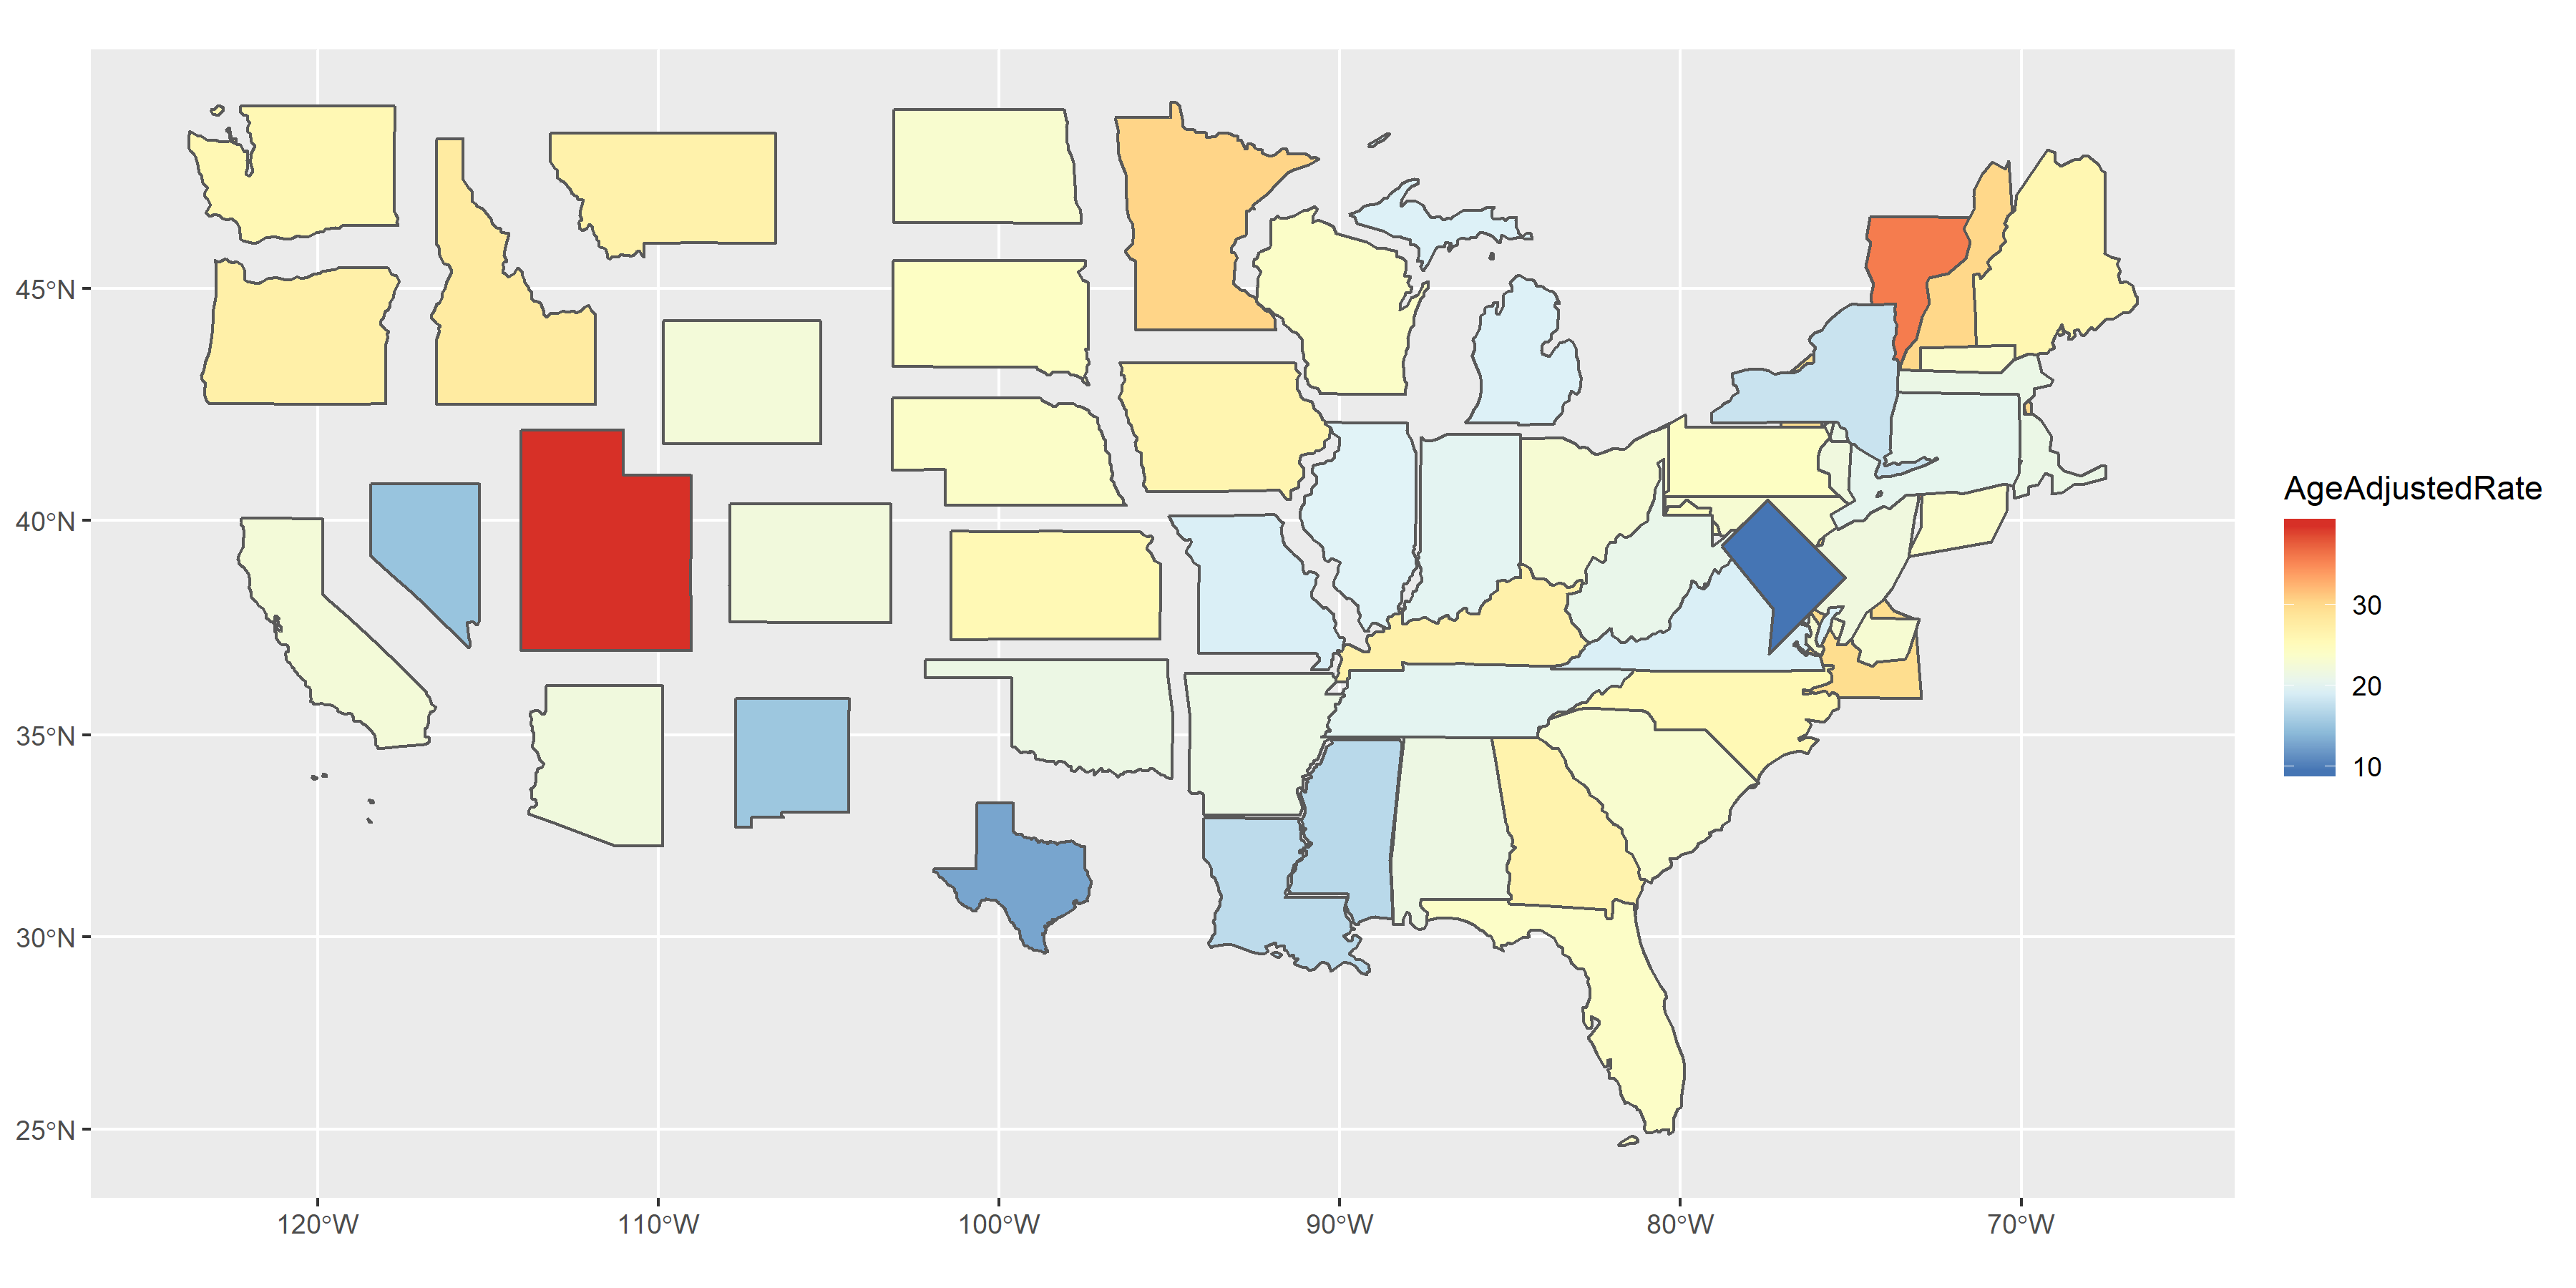
\includegraphics{figures/ggncont.png}
\caption{``A Non - contiguous cartogram of the Unites States of
America''}
\end{figure}

\begin{figure}
\centering
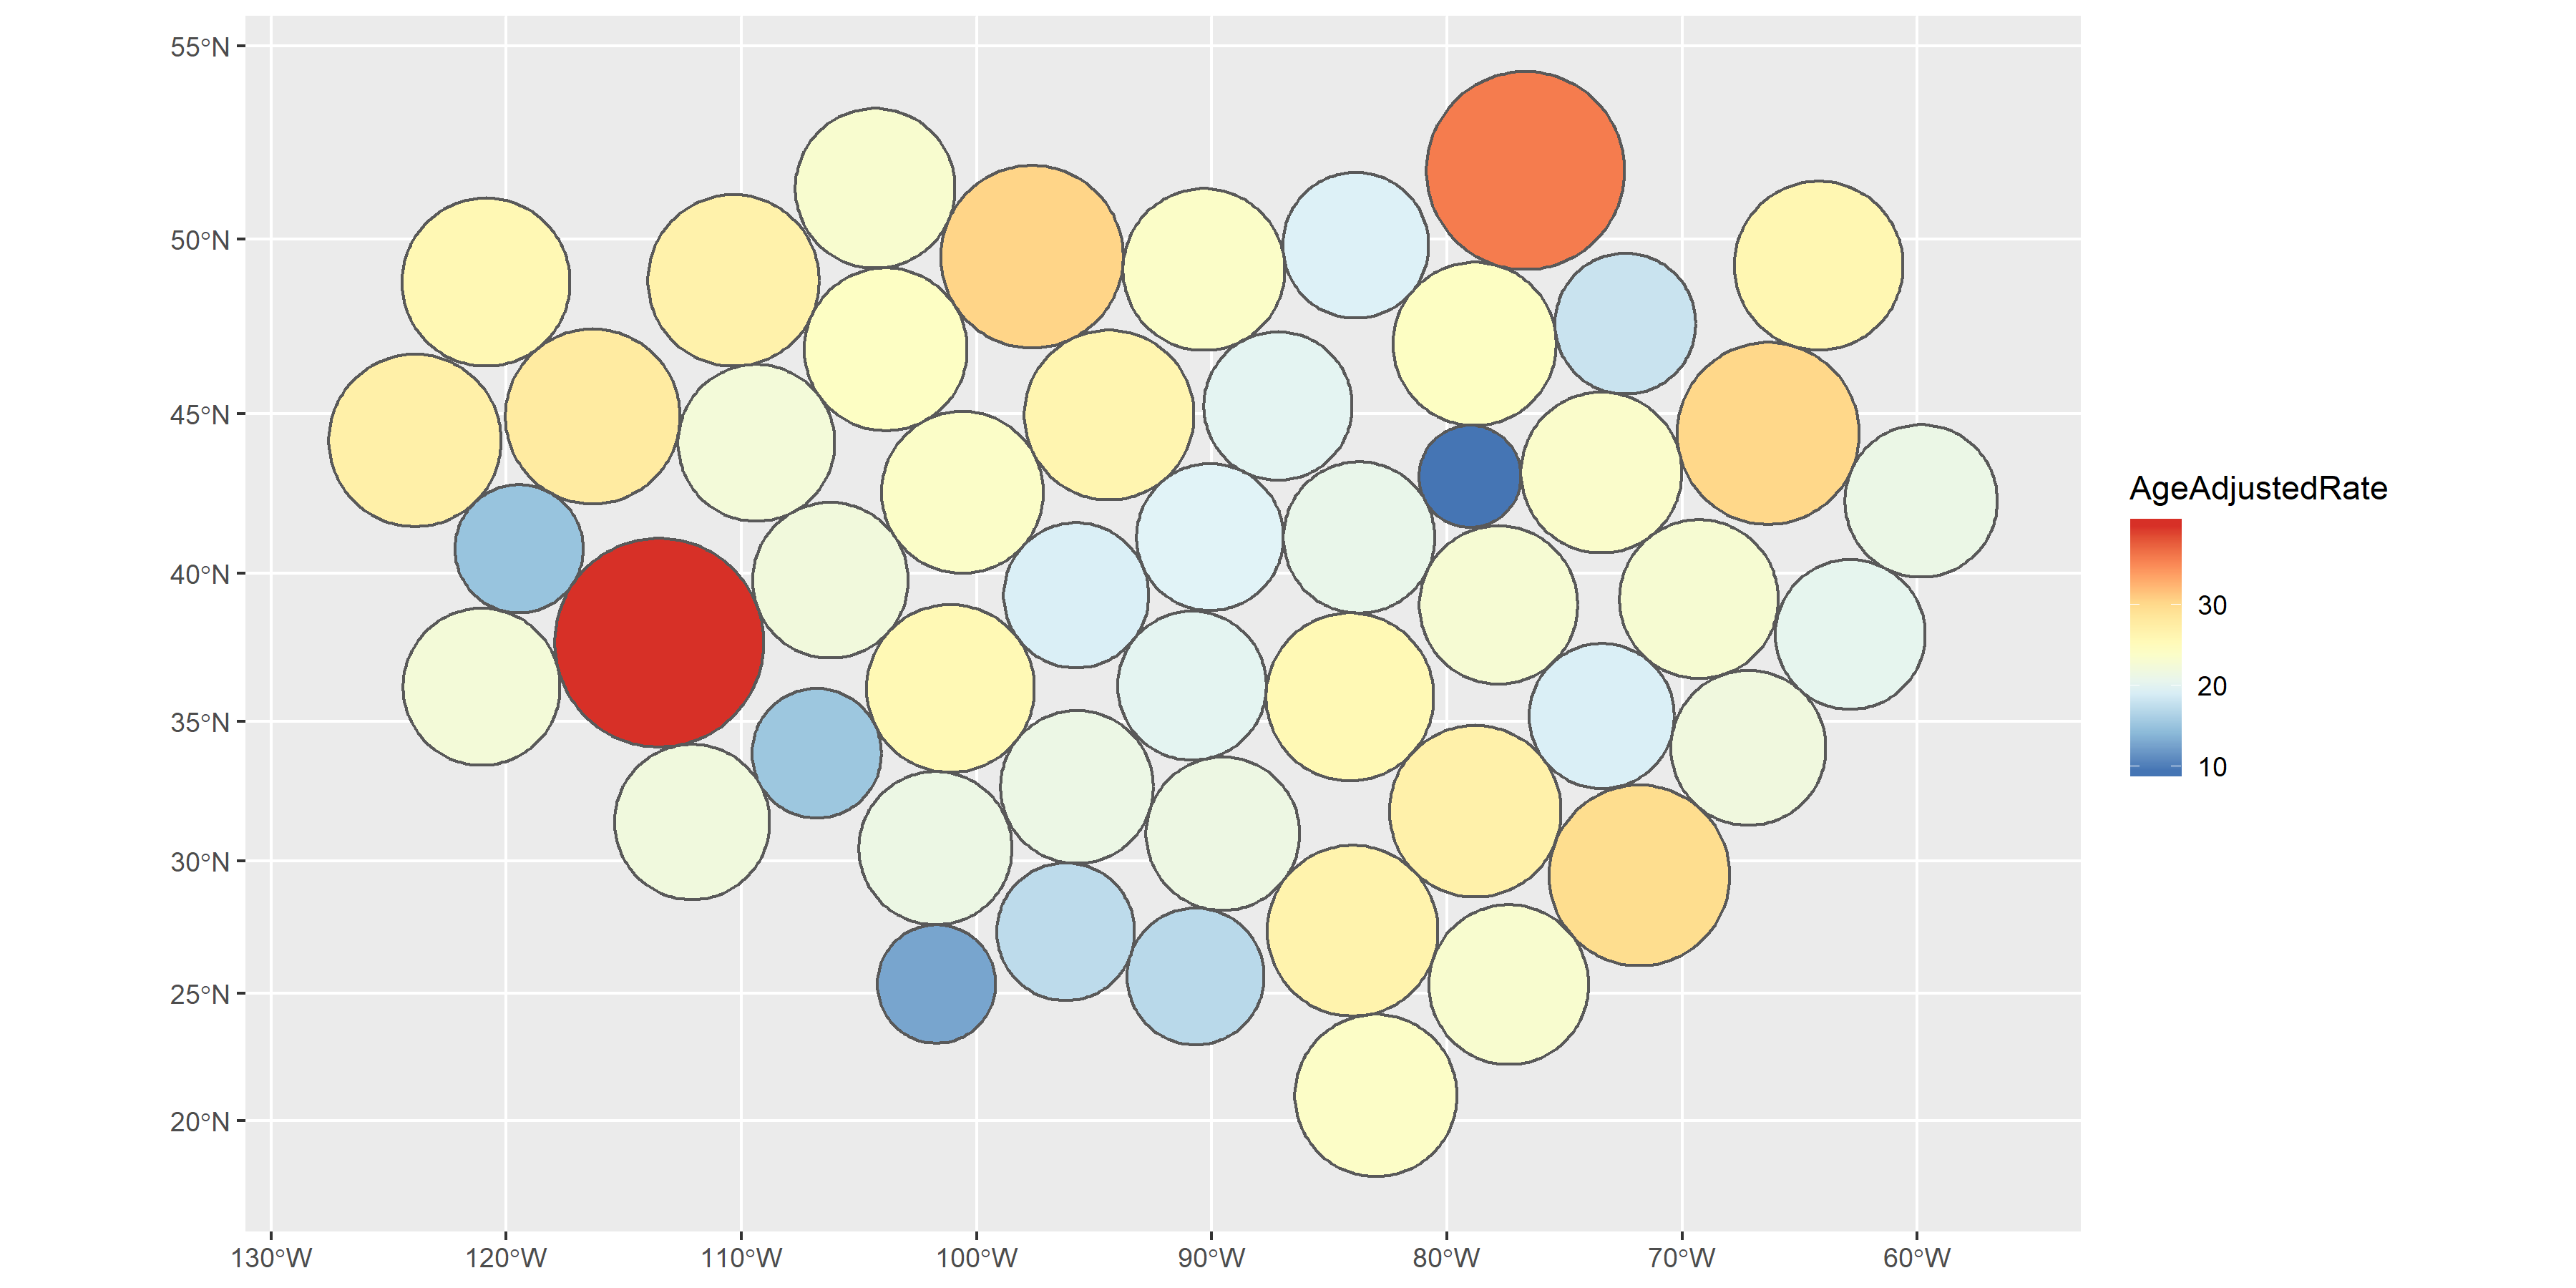
\includegraphics{figures/ggdorl.png}
\caption{``A dorling cartogram of the Unites States of America''}
\end{figure}

Dorling (\protect\hyperlink{ref-ACTUC}{2011}) puts forward a simple
question:

\begin{quote}
If, for instance, it is desirable that areas on a map have boundaries
which are as simple as possible, why not draw the areas as simple shapes
in the first place?
\end{quote}

He answers this with his implementation of maps created with `the
simplest of all shapes'. While contiguous cartograms may be a `more
sophisticated' method, they produce `very complex shapes'. Circular
cartograms use the same shape for every region represented, and size
them according to the statistic represented or the population for a base
map. To produce a compelling map, a gravity model is applied to avoid
overlaps, and keep spatial relationships with neighbouring areas over
many iterations. This implementation can work for up to `one hundred
thousand' areas.

Dorling (\protect\hyperlink{ref-ACTUC}{2011}) suggests `population
distribution is often extremely uneven in former British colonies'.

`In Australia the urban federal constituencies occupy only a tenth of
the land, but contain nine tenths of the people. It would be almost
unthinkable to show election results for that country on a conventional
equal land area map.' This 1966 cartogram uses mostly straight lines,
and the result looks very little like the geographical shape of
Australia.

`Given the increasingly uneven population distribution of the United
States and the growing social divides between the populations of
neighbourhoods living at different densities, the need for cartograms
like this is greater now than ever.'

Used in displays of the UK by Howe in 1986 cited by Howe
(\protect\hyperlink{ref-HEDP}{1989})

Tobler's method and the many implementations that `elaborated' on it are
derived from `numerical approximations to a pair of equations'(Dorling
\protect\hyperlink{ref-ACTUC}{2011}). They all operate through
incremental adjustments, and can produce wildly different outcomes from
small changes in the inputs.

Tobler (\protect\hyperlink{ref-TFYCC}{2004}) Value-Area Cartograms. In
these cartograms a region,country, or continent is subdivided into small
regions, each of which is represented by a rectangle. This rectangle is
proportionate in area to the value which it represents in certain
statistical distributions. The regions are grouped in approximately the
same positions as they are on the map.

Computer generated map examples: Howe
(\protect\hyperlink{ref-HEDP}{1989}) (Hopps et al.~1968; Armstrong
1972). There has followed a flood of disease atlases, mainly
concentrating on the modem problems of cancer and degenerative diseases
from countries as scattered as the United States (Burbank 1971; Mason et
al.~1975, 1976; Pickle et al.~1987), the Soviet Union (Levin 1980),
Japan (Shigematsu 1977), the Federal Republic of Germany

Cano et al. (\protect\hyperlink{ref-MDAC}{2015}) define the term `mosaic
cartograms'. Compare amount of tiles to contrast population of regions.
`Cartograms show a data value per input region by scaling each region
such that its area is proportional to its data value. Mosaic cartograms
show data in multiples of tiles, hence the input data must consist of,
or be cast into, small integer units.'

\hypertarget{centroid-displays}{%
\subsection{Centroid displays}\label{centroid-displays}}

Dot plot: one dot for each region, coloured, and placed at centroid.

Olson (\protect\hyperlink{ref-NAC}{1976}) gives an example of

Plotting centroids on top of geographies. (Size is kept constant)

Replies on the idea that every area is important, no matter the size.
This gives equal emphasis to every area, allows distributions and
relationships between neighbours to become more clear.

\hypertarget{a-critique-of-mapping-methods}{%
\section{A critique of mapping
methods}\label{a-critique-of-mapping-methods}}

\begin{quote}
designing a map tailored to precise goals {[}is{]} easier than forcing a
single map to accommodate diverse objectives - Bell et al.
(\protect\hyperlink{ref-CPISACA}{2006})
\end{quote}

With that in mind, the intended user and message to communicate should
drive map selection. first is the nature or inherent properties of the
device itself second is the ease and accuracy with which map users are
able to extract information from it

Moore and Carpenter (\protect\hyperlink{ref-SAMGIS}{1999}) suggests it
is the ``investigators' objectives'' that drive the ``representation of
diseases on maps''. -infectious diseases may require choropleth methods

`Where control of the message is important, static maps will continue to
be the most effective, although good tables, graphs, and explanatory
text are still needed in order to ensure that different people will see
the same thing in the maps' Bell et al.
(\protect\hyperlink{ref-CPISACA}{2006})

(only worth including if it is possible for us to implement) Tabular
form comparing and contrasting - Relationship to geography

\begin{itemize}
\tightlist
\item
  Show using cancer examples
\end{itemize}

\hypertarget{animation}{%
\section{Animation}\label{animation}}

lends to temporal pattern exploration

Keim et al. (\protect\hyperlink{ref-ECGC}{2002}) ?? Highlight the value
of animating contiguous to see changes over time, US can be recognisable
but animation aides interpretation

\hypertarget{acknowledgements}{%
\section{Acknowledgements}\label{acknowledgements}}

What software did we use, for e.g.

\hypertarget{references}{%
\section{References}\label{references}}

\hypertarget{refs}{}
\leavevmode\hypertarget{ref-CPISACA}{}%
Bell, B Sue, Richard E Hoskins, Linda Williams Pickle, and Daniel
Wartenberg. 2006. ``Current Practices in Spatial Analysis of Cancer
Data: Mapping Health Statistics to Inform Policymakers and the Public.''
\emph{International Journal of Health Geographics} 5: 49.
\url{https://doi.org/10.1186/1476-072X-5-49}.

\leavevmode\hypertarget{ref-GOINO}{}%
Berry, Brian J. L., Richard L. Morrill, and Waldo R. Tobler. n.d.
``GEOGRAPHIC Ordering of Information: NEW Opportunities'' 16 (4).
Association of American Geographers: 39--44.
\url{https://doi.org/10.1111/j.0033-0124.1964.039_q.x}.

\leavevmode\hypertarget{ref-CIBMUK}{}%
Brewster, Mark B., and S. V. Subramanian. 2010. ``Cartographic Insights
into the Burden of Mortality in the United Kingdom: A Review of `The
Grim Reaper's Road Map'.'' Journal Article. \emph{International Journal
of Epidemiology} 39 (4): 1120--2.
\url{https://doi.org/10.1093/ije/dyp395}.

\leavevmode\hypertarget{ref-MDAC}{}%
Cano, R. G., K. Buchin, T. Castermans, A. Pieterse, W. Sonke, and B.
Speckmann. 2015. ``Mosaic Drawings and Cartograms.'' \emph{Computer
Graphics Forum} 34 (3): 361--70.

\leavevmode\hypertarget{ref-ACTUC}{}%
Dorling, Daniel. 2011. ``Area Cartograms: Their Use and Creation.'' In
\emph{Concepts and Techniques in Modern Geography (CATMOG)}, 59:252--60.
\url{https://doi.org/10.1002/9780470979587.ch33}.

\leavevmode\hypertarget{ref-TVSSS}{}%
---------. 2012. \emph{The Visualisation of Spatial Social Structure}.
John Wiley \& Sons Ltd.

\leavevmode\hypertarget{ref-SE}{}%
Exeter, Daniel J. 2017. ``Spatial Epidemiology.'' Journal Article, 1--4.
\url{https://doi.org/10.1002/9781118786352.wbieg0283}.

\leavevmode\hypertarget{ref-CTTMB}{}%
Griffin, T.L.C. 1980. ``Cartographic Transformation of the Thematic Map
Base.'' \emph{Cartography} 11 (3). Taylor \& Francis: 163--74.
\url{https://doi.org/10.1080/00690805.1980.10438102}.

\leavevmode\hypertarget{ref-HEDP}{}%
Howe, G. M. 1989. ``Historical Evolution of Disease Mapping in General
and Specifically of Cancer Mapping.'' In \emph{Cancer Mapping}, edited
by Peter Boyle, Calum S. Muir, and Ekkehard Grundmann, 1--21. Berlin,
Heidelberg: Springer Berlin Heidelberg.

\leavevmode\hypertarget{ref-MTMSIH}{}%
Jahan, Farzana, Earl Duncan, Susanna Cramb, Peter Baade, and Kerrie
Mengersen. 2018. ``Making More of Spatial Maps: A Bayesian Meta-Analysis
Approach.'' In.

\leavevmode\hypertarget{ref-ECGC}{}%
Keim, D.A, S.C North, C Panse, and J Schneidewind. 2002. ``Efficient
Cartogram Generation: A Comparison.'' In \emph{IEEE Symposium on
Information Visualization, 2002. INFOVIS 2002}, 2002-:33--36. IEEE.

\leavevmode\hypertarget{ref-CBATCC}{}%
Kocmoud, Christopher J., and Donald H. House. 1998. ``A Constraint-Based
Approach to Constructing Continuous Cartograms.'' In.

\leavevmode\hypertarget{ref-TAAM}{}%
Levison, M. E., and W. Haddon Jr. 1965. ``THE Area Adjusted Map. AN
Epidemiologic Device.'' Journal Article. \emph{Public Health Reports}
80: 55--59.

\leavevmode\hypertarget{ref-ACA}{}%
Min Ouyang, and P. Revesz. 2000. ``Algorithms for Cartogram Animation.''
In \emph{Proceedings 2000 International Database Engineering and
Applications Symposium (Cat. No.PR00789)}, 231--35.
\url{https://doi.org/10.1109/IDEAS.2000.880581}.

\leavevmode\hypertarget{ref-SAMGIS}{}%
Moore, Dale A., and Tim E. Carpenter. 1999. ``Spatial Analytical Methods
and Geographic Information Systems: Use in Health Research and
Epidemiology.'' \emph{Epidemiologic Reviews} 21 (2): 143--61.
\url{https://doi.org/10.1093/oxfordjournals.epirev.a017993}.

\leavevmode\hypertarget{ref-SAIC}{}%
Nusrat, Sabrina, and Stephen G. Kobourov. 2016. ``The State of the Art
in Cartograms.'' \emph{CoRR} abs/1605.08485.
\url{http://arxiv.org/abs/1605.08485}.

\leavevmode\hypertarget{ref-NAC}{}%
Olson, Judy M. 1976. ``NONCONTIGUOUS Area Cartograms.'' \emph{The
Professional Geographer} 28 (4). Routledge: 371--80.
\url{https://doi.org/10.1111/j.0033-0124.1976.00371.x}.

\leavevmode\hypertarget{ref-GAMP}{}%
Tobler, Waldo. 1963. ``Geographic Area and Map Projections,'' January.
American Geographical Society, 59--78.
\url{https://www.jstor.org/stable/212809}.

\leavevmode\hypertarget{ref-TFYCC}{}%
---------. 2004. ``Thirty Five Years of Computer Cartograms.''
\emph{Annals of the Association of American Geographers} 94 (1). Taylor
\& Francis Group: 58--73.

\leavevmode\hypertarget{ref-EI}{}%
Tufte, Edward R. 1990. \emph{Envisioning Information}. Graphics Press.

\leavevmode\hypertarget{ref-DMAHP}{}%
Walter, S. D. 2001. \emph{Disease Mapping: A Historical Perspective}.
Book. Oxford University Press: Oxford.


\end{document}
